\documentclass{llncs}
\usepackage[latin1,utf8x]{inputenc}
\usepackage{color}
\usepackage[pdftex]{graphicx}
\usepackage{amsmath}
\usepackage{verbatim}
\usepackage{marginnote} 
%\usepackage[outer=5cm, inner=2cm, heightrounded, marginparwidth=4cm, marginparsep=0.5cm]{geometry}

\newcommand\margin[1]{\marginnote{\scriptsize{\bfseries #1}}}

\pagestyle{plain}


\title{Classification Techniques for Conformance and Performance checking in Process Analysis}
\author{Hind Chfouka, Andrea Corradini, Roberto Guanciale}
\institute{Department of Computer Science, Università di Pisa}
\date{today}
\begin{document}
\maketitle
\begin{abstract}
Standard process analysis techniques like conformance checking or performance evaluation are enabled by the event logs that trace the process executions and by the presence of a model that formally represents the process. Such analysis techniques use only part of the huge amount of data recorded in the event logs. In this paper the goal is to transform this data into useful information for the conformance checking and the performance analysis. Through classification technique, we present an approach to investigate how the process data influences its behavior in term of conformance and performance. 
\end{abstract}

\section{Introduction}
Today, many Information Systems that integrate the concept of business process record all events occurring during the process execution in an event log. An event log represents a trace of the process behavior that can be observed and analyzed in order to tune it with the business objectives pursued. Process Mining provides a set of techniques for process discovery and analysis. Through the knowledge extracted from event logs, process discovery allows the construction of a process model. Process analysis instead assumes the existence of a model and it consists of checking the conformance and performance of the process executions with respect to it.

The motivation of this paper is based on the observation that existing event logs are rich of data, and this data is used only in part by the existing process analysis techniques. Since data is considered a valid source of knowledge, developing a technique based on data analysis can provide advantages for  process analysis.
Therefore, our goal consists of finding a way for transforming the data recorded during the process activities in knowledge useful for the analysis. To this aim, one possible approach is to try to understand how data may influence the process behavior. In particular, it is interesting to understand how may the data influence the conformance and performance of the process executions. Exploring this influence can provide qualitative information about the causes of possible anomalies in the process behavior, facilitating the task of taking corrective measures.

In order to analyze data arising from event logs, in this paper we present an approach based on \emph{data mining} \cite{5}. In particular, we exploit \emph{classification} techniques to find patterns on data in presence of which conformance errors occur. Next, the same approach is extended to consider the process behavior in terms of performance to discover how data influences the process efficiency. Classification is a well-known \emph{machine learning} technique, and it consists of identifying to which category among a given set a new observation belongs. This is done on the basis of a training set of data containing observations whose category membership is known.

Classification techniques in the Process Mining field have already been explored. In \cite{1} the idea is exploring how data influences the case routing of process flow execution. In this contribution the goal is to strengthen the use of data analysis techniques for the benefit of process analysis. This is done by studying how data may influence, in general, the overall process behavior.

After the presentation of a case study in Section \ref{example},
Section \ref{Background} introduces some background concepts about
process analysis. First the algorithm log replay is briefly described,
then conformance and performance analysis are presented. Both kind of
analysis are illustrated through the business process of Section
\ref{example}. In Section \ref{ClassifApproach} our approach to
process analysis based on classification is presented. First a few
basic concepts about the classification technique are described, next
the conformance analysis based on classification is presented in
detail through an illustration with our case study, moreover a
possible extension of the approach for performance analysis is
presented. Finally, Section \ref{implementation} describes the
implementation of our approach provided as \emph{ProM6}\cite{6} plug-ins, as well the methodology to follow in the process analysis based on classification.

\section{The case study: a sale business process}\label{example}
A business process can be seen as a collection of activities occurring within an organization that lead to a specific goal. There are several formalisms for representing business processes. In this paper we represent them using Petri nets \cite{8}\cite{10} since this make possible exploiting some existing process analysis techniques that are based on Petri nets. However, in the business management context, Petri nets can be not expressive enough and usually process models are presented as flowcharts, in particular using the standard for the business process modeling: BPMN (Business Process Model and Notation) \cite{9}. Transforming a BPMN model into a Petri net is possible thanks to a mapping technique presented in \cite{12}\cite{2}.
\begin{figure}[h]
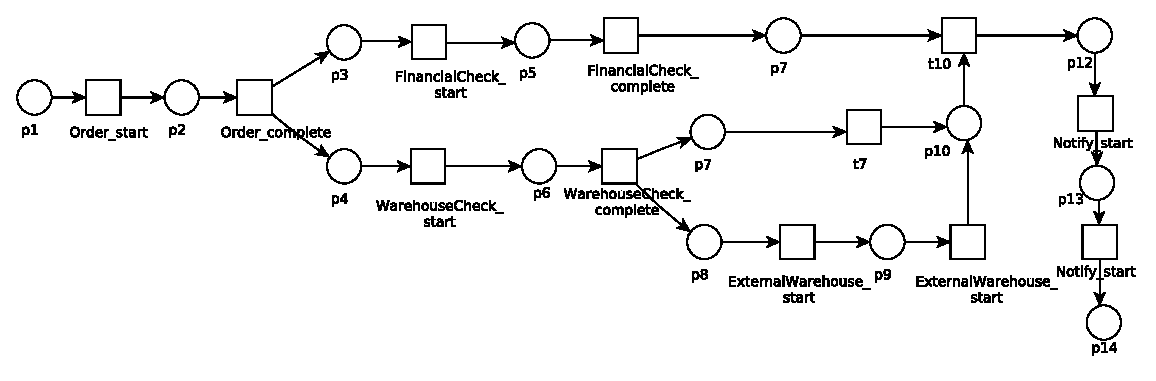
\includegraphics[width=360pt]
{./items/Sales_PN.pdf}
\caption{Petri net for a a sale process}
\label{pnet}
\end{figure}

Figure \ref{pnet} presents the Petri net model for a sale
process.
\footnote{
The Petri net of Figure \ref{pnet} is obtained by
transforming a BPMN model using the algorithm of \cite{2}, and mapping
each activity to a pair of start/end transitions. The resulting net
has been simplified by removing the unnecessary \emph{invisible
  transitions} used to encode the \emph{Join} or \emph{Fork} gateway \cite{2}.
}
This business process abstractly represents a fragment of the
procedure followed in a commercial organization for managing orders
received from clients. In general this procedure includes several
activities and each of them involves a specific department of the
organization. We assume that the sale process begins with the
notification of an order from a client, so the first activity is
simply called \emph{Order}. After the order is received, the sale
process continues with some activities that can be done in parallel,
since they do not present any dependencies. The \emph{FinancialCheck}
activity represents the financial analysis of the order  (i.e
verifying the financial situation of the client). Concurrently, the
\emph{WarehouseCheck} activity checks the availability of merchandise
requested by the order and, in case of a shortage, starts a supplying procedure. This is done through the activity \emph{ExternalWarehouse}. After the completion of the  parallel activities, a synchronization is needed before continuing the sale procedure with the final activity called \emph{Notify}, by which a result regarding the acceptance of the order is communicated to the client.

<<<<<<< HEAD
Note that the Petri net of Figure \ref{pnet} is obtained by transforming a BPMN model using the algorithm described in \cite{2}, and mapping each activity to a pair of start/end transitions. The resulting net has been simplified by removing the unnecessary \emph{invisible transitions} used to encode e.g. the \emph{Join} or \emph{Fork} gateway \cite{2}.

\section{Process Analysis}\label{Background}
%Process analysis is performed using the Petri net representing the process and an event log recording the related executions, also called \emph{process instances}. The basic building blocks of event logs are events. An event {\itshape e} can be seen as a pair {\itshape e = (a,t) } representing an action {\itshape a } recorded and the corresponding timestamp {\itshape t}. Action and timestamp are denoted respectively by $\alpha(e)$ and $\phi(e)$. Events that belong to the same process are grouped into {\itshape traces}. Formally, a trace $T$ is a finite sequence of events $T[1],..., T[n]$, such that $\phi(T[i]) \leq \phi(T[i+1])$ for all  $i \in [1,n)$. A log $L$ is a set of traces, recording the activities performed by a system during a finite number of process executions.
Process analysis is performed using the Petri net representing the process and an event log recording the related executions, also called \emph{process instances}. The basic building blocks of event logs are events. An event $e$ can be seen as a pair $e = (a,t)$ representing an action $a$ recorded and the corresponding timestamp $t$.  Events that belong to the same process are grouped into {\itshape traces}. A trace $T$ is a finite sequence of events ordered based on timestamp. A log $L$ is a set of traces, recording the activities performed by a system during a finite number of process executions.  In this paper the following assumptions are made:
\begin{itemize}
\item All traces are instances of the same process.
\item For each action there exist two corresponding transitions in the net that will be denoted, for simplicity, by the same name of the action.
\end{itemize}
=======

\section{Process Analysis}\label{Background}

Process analysis is performed using the Petri net representing the
process and an event log recording the related executions, also called
\emph{process instances}. The basic building blocks of event logs are
events. An event {\itshape e} can be seen as a pair {\itshape e =
  (a,t) } representing an action {\itshape a } observer at the
timestamp {\itshape t}. Action and timestamp are denoted respectively
by $\alpha(e)$ and $\phi(e)$. Events that belong to the same process
are grouped into {\itshape traces}. Formally, a trace $T$ is a finite
sequence of events $T[1],..., T[n]$, such that $\phi(T[i]) \leq
\phi(T[i+1])$ for all  $i \in [1,n)$. A log $L$ is a set of traces,
recording the activities performed by a system during a finite number
of process executions. In this paper we assume that
(i) all traces are instances of the same process
and
(ii) for each action there exists a corresponding transition (labeled
with the same name of the action) in the Petri net.
>>>>>>> guancio

\subsection{Log replay algorithm}\label{logreplayAlg}
The key algorithm exploited to analyze a Petri net model with respect to the log is the {\itshape log replay} algorithm \cite{13}\cite{3}\cite{4}. Given a Petri net model and an event log as input to the algorithm, the output results can be used to check the conformance of traces and to evaluate some performance metrics. For each trace in the log, the algorithm starts by placing one token in the start place of the net. For each event in the trace the corresponding transition is fired assuming a {\itshape non-blocking} behavior of the algorithm, then the marking of the net is updated. Non-blocking replay means that whenever a firing of a disabled transition is needed, the algorithm enables the transition either creating artificial tokens in the pre-set or, if possible, firing some invisible transitions; the non-determinism in this procedure is resolved with a suitable cost function. %The output of a log replay execution on a trace can be represented as an ordered list $R$ of pairs $(tr, i)$, representing that the transition $tr$ has been fired to mimic the event $T[i]$.

% The log replay result can be used to evaluate both the conformance and performance of a business process. 

\subsection{Conformance Analysis}\label{ConformanceAnalysis}
The goal of the conformance analysis is to check if a trace complies with the Petri net modeling the business process. Conformance problems can be discovered by analyzing tokens artificially created during the replay {\itshape (the missing tokens)} and tokens not consumed {\itshape (the remaining tokens)}. Figure \ref{ConfLog}  presents two different traces, $T$ and $T'$, of the business process presented in Section \ref{example}. The log replay of the trace $T$, which is compliant with the Petri net, terminates with a marking containing one token in the end place \{${p13 \rightarrow 1}$\} and without reporting any missing tokens.

\begin{comment}
\begin{equation}
\begin{split}
R&=\{(Order\_start,1), (Order\_complete,2),(WarehouseCheck\_start,3), \\
& (FinancialCheck\_start,4),(FinancialCheck\_complete,5),\\
& (WarehouseCheck\_complete,6),(t2, 7), (Notify\_start,7), \\
&(Notify\_complete,8)\}
\end{split}
\end{equation}
\end{comment}

\begin{figure}[h]
\centering
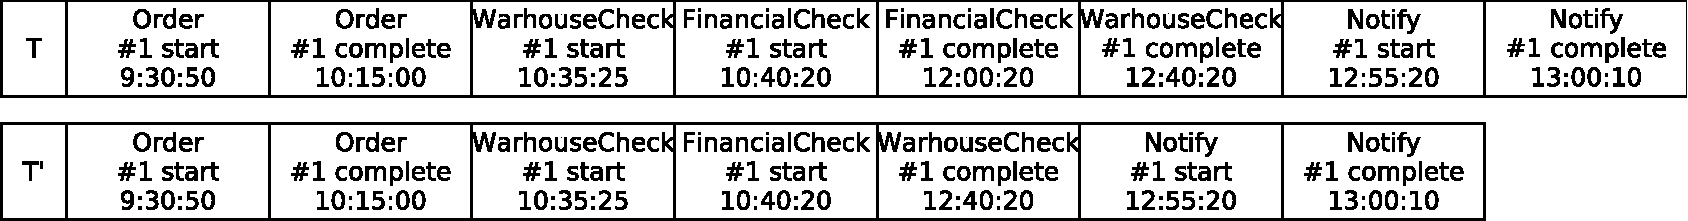
\includegraphics[width=0.9\linewidth]
{./items/logConforme.pdf}
\caption{Conform ($T$) and non-conform ($T'$) traces}
\label{ConfLog}
\end{figure}


The log replay of the trace $T'$ terminates with remaining tokens \{$p5 \rightarrow 1$, $p13 \rightarrow 1$\} and one missing token \{${p8 \rightarrow 1}$\}. The missing token is created artificially and this fact witness a wrong execution of the event $Notify\_start$. In fact, in $T'$ this event is executed before the termination of the activity \emph{FinancialCheck}: this is interpreted as a non-conformance to the process model. 

\begin{comment}
The sequence returned by log replay is:
\begin{equation}
\begin{split}
R'&=\{(Order\_start,1), (Order\_complete,2), (WarehouseCheck\_start,3), \\
& (FinancialCheck\_start,4), (WarehouseCheck\_complete,5),(t1,6),(t2,6),\\
& (Notify\_start,6), (Notify\_complete,7)\}
\end{split}
\end{equation}
\end{comment}



\subsection{Performance analysis}\label{PerformanceAnalysis}
The performance of a process can be analyzed by exploiting the log
replay results. Since the logs contain timestamps, the log replay can
be used to compute performance measures of the process my measuring the elapsed time between production and consumption of tokens. Performance analysis can be applied only to traces that do not generate missing tokens during the replay since such tokens cannot have time information \cite{2} . During the log replay the following metrics can be computed for each trace and each place:
\begin{itemize}
\item sojourn time $(tsj)$ : the time interval between arrival and departure of tokens;
\item synchronization time $(tsc)$: the time interval between arrival of a token in the place and enabling of a transition in the post-set of the place;
\item waiting time $(tw)$:  the time interval between enabling of a transition in the post-set of the place and token departure (thus $tsj=tsc+tw $).
\end{itemize}

The duration of an activity is an important performance measure as well, and it is given by the waiting time of the only place between the start and the complete transition of the activity.

\begin{comment}
To clarify the metrics evaluated by this technique, as done with conformance analysis, we exploit the Petri net  presented in Section \ref{example} and the trace T presented in Figure \ref{ConfLog}. The replay starts with firing the transition $Order\_start$ at time $0s$, so a token arrives at $p2$ at time $0s$. After $45 min$ the token in $p2$ is consumed and the transition $Order\_complete$ is fired, so $tw(p2)=45min$, and a token arrives at $p3$ and $p4$. At the time $1h:5min:25s$ the transition $WarhouseCheck\_start$ is fired, thus $tw(p4)=20min+25sec$ and a token is produced at $p6$. At the time $1h:10min:20s$ the transition $FinancialCheck\_start$ is fired and a token is produced at $p5$, so $tw(p3)=25min+20s$. After $2h:30min:20s$ from the replay start the transition $Financial\_complete$ is fired, hence we have $tw(p5)=1h+20min$ and a token is produced at $p8$. At time $3h:10min:20s$ the firing of the transition $WarehouseCheck\_complete$ is executed, so $tw(p6)=2h+4min+55s$ and a token is produced at $p7$. After $15 min$ the invisible transition $t1$ is fired and a token is produced at $p10$. At this point the transition $t2$ is enabled, so its firing is now possible and a token is produced at $p11$. Notice that $tsc(p8)=40min, tsc(p10)=0s$. At the time $3h:25min:20s$ the transition $Notify\_start$ is fired and a token is produced in $p12$, after $4min+4sec$ the transition $Notify\_complete$ is fired and $tw(p12) = 4min+40s$.

It is worth noting that the synchronization time is greater than zero
only for places which contain in their post-set transitions depending
from other places. For the Petri net in Figure~\ref{pnet}, the only
places which can have a non-null synchronization time are $p8$ and
$p10$. For example, the synchronization time is greater than zero for
$p8$ in the trace $T$ in Figure \ref{ConfLog}, representing that, for
this particular process instance, the branch performing the financial
checking is faster than the warehouse branch.

\end{comment}


\section{An approach based on classification for Process Analysis}\label{ClassifApproach}
Employing data mining techniques for process analysis is encouraged by the presence of a huge amount of data recorded in event logs under \emph{attribute} format. The implicit information contained in those data could be significant for the process behavior analysis. In fact, this potential information could contain an explanation for the deviations discovered during conformance analysis, and for the performance level provided by the process. For this reason, we are interested in discovering how the process data may influence the conformance and the performance of the process executions. This is done with an approach based on \emph{classification}, a classical data mining technique able to detect patterns on data in correspondence to which the process assumes a specific behavior.

\subsection{Classification: basic concepts}\label{classifBasicConcept}

In a classification problem \cite{5}, data is represented by a
collection of records (called instances), and each of them is
characterized by a tuple $(\mathbf{x},y)$, where $\mathbf{x}$ is a set
of attributes and $y$ is a special attribute called \emph{target attribute}. The target denotes the class to which a record belongs. The goal is to learn a classification model that maps each attribute set $\mathbf{x}$ to one of the predefined class labels $y$.

A classification model can be useful for a descriptive purpose: it provides an explanatory tool to distinguish between objects of different classes, and for a predictive purpose: the model can be used to predict the class label of new records. In this way the model acts as a black box that automatically assigns a class label to an attribute set of a new record.

There is a general approach to solve a classification problem from a dataset, that is independent from the specific classification model. Each classification technique employs a learning algorithm to identify a model that best fit the relationship between the attribute set and class label of the input data. The model generated should both fit the input data well, and correctly predict the class labels of new records. Finding the right trade-off between this two purposes is the most delicate part of a classification technique, and in general of any machine learning task.

\begin{figure}[h]
\centering
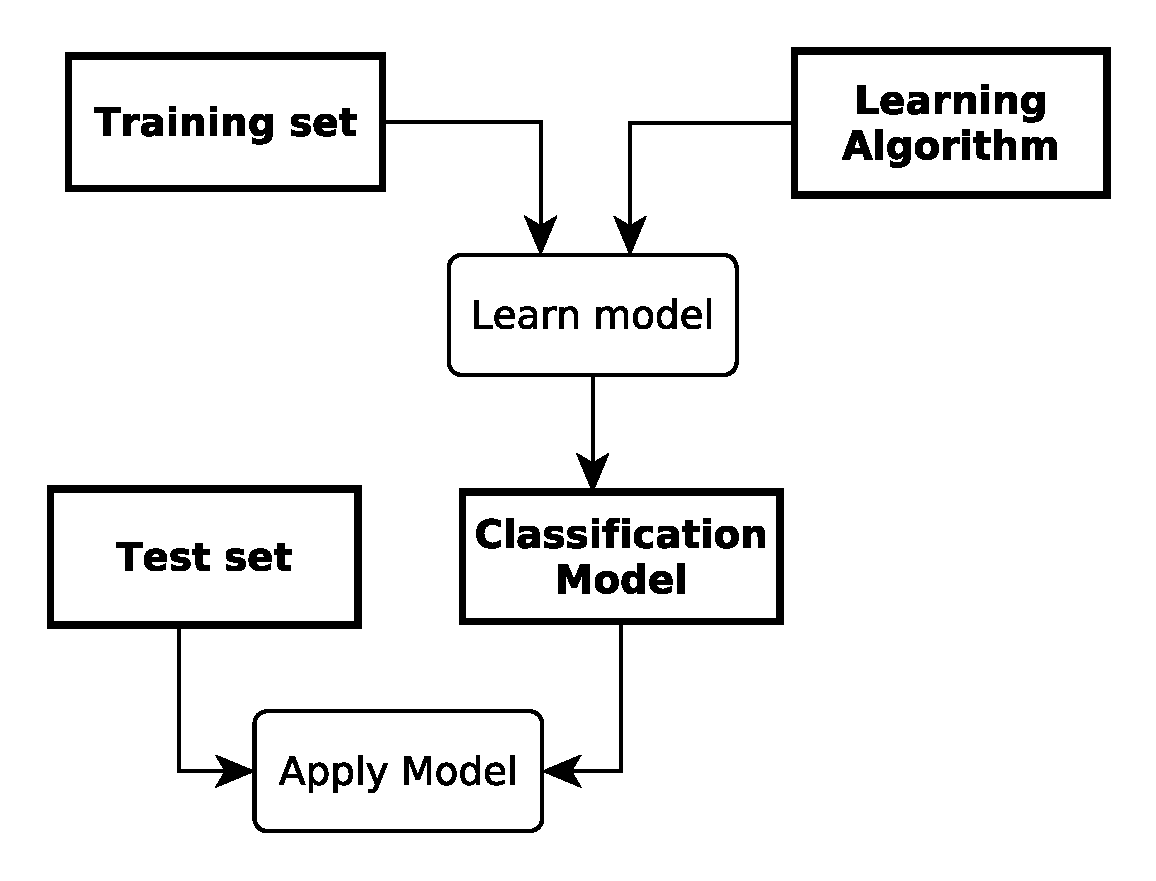
\includegraphics[width=200pt]
{./items/classifApproach.pdf}
\caption{General approach for solving a classification problem.}
\label{figclassApproach}
\end{figure}

Figure \ref{figclassApproach} summarizes the general approach for solving a classification problem \cite{5}. A \emph{Training set} consisting of records whose class labels are known must be provided to a learning algorithm, and it is used to build a classification model. This model is then applied to a \emph{test set}, which consists of records with unknown class labels. This application allows the estimation of the \emph{model accuracy} that can be done in different ways. The simple one consists in computing the accuracy as the number of the records correctly predicted over the total number of records in the test set.

Many classification models could be used for a classification problem. For our purpose we choose the \emph{decision tree} model since the rules detected by the classification are shown explicitly. This fact is fundamental for giving an explanation to the process behavior based on the process data values. Furthermore, this choice is encouraged by the simplicity of decision trees. In a decision tree, a class label (possible value of the attribute target) is assigned to each leaf node. The non-terminal nodes, which include the root and the internal nodes, contain attribute test conditions to filter records that have different characteristics.
\begin{comment}
In principle, there are exponentially many decision trees that can be constructed from a given set of attributes. While some of the trees are more accurate than others, finding the optimal tree is computationally infeasible because of the exponential size of the search space. However, efficient algoritms have been developed to induce a reasonably accurate decision tree in a reasonable amount of time. These algorithms usually employ a greedy strategy that grows a decision tree by making a series of decisions about which attribute to use for partioning the data. For instance Hunt's algorithm is one of them and it represents the basis of many existing decision tree induction algorithms, including $C4.5$ algorithm used for our purposes.
\end{comment}
\subsection{Classification for Conformance Checking}\label{ClassConformance}
In order to identify the possible causes of non-conformance, a classification problem can be formulated. The classification dataset is extracted from the process data: for each process instance, one will extract some data that will be included as a record in the dataset. For the process presented in Section \ref{example}, a record is characterized by the following attribute set: an instance identifier, a client identifier, the client typology (new or consolidated client), the sales manager responsible for the order, the financial officer who conducts the financial evaluation activities, the warehouseman responsible for the warehouse checking, the supplying responsible name in case of a provision, and finally the result communicated to the client for the order issued. The conformance result for the process instance provides an additional and important data which takes the role of the target attribute. All these attributes are discrete and contribute to build the dataset presented in Table \ref{tab:SaleData} of the classification problem. Note that, since the goal of this paper is just to illustrate an approach for exploiting process data in the process analysis, the data presented here is just a synthetic data that was generated with some noise to emulate a real situation.

\begin{table}[!h]
\scriptsize{
\centering
\begin{tabular}{|p{1cm}|p{1cm}|p{1,5cm}|p{1,2cm}|p{1,4cm}|p{1,2cm}|p{1,5cm}|p{1,4cm}|p{0,8cm}|}
\hline OrdIde & CltIde & CltType & SalMan & FinOff & WrhsMan & SupplyResp & OrdResut & Conf\\
\hline
1 & 20 & consolidate & Marco & Mary & Alex & Gianni & positive & no\\
\hline
2 & 15 & new & Anna & Johann & Roberto & Mario & positive & yes\\
\hline
3 & 10 &consolidate & Maria & Mary & Alessio & Gianni & negative & no\\
\hline
10 & 18 & consolidate & Johann & Mary & Roberto & Gianni & positive & yes \\
\hline
... & ... & ... & ... & ... & ... & ... & .... & ...  \\
\hline
\end{tabular}
}
\caption{Dataset for the conformance analysis.}
\label{tab:SaleData}
\end{table}
\normalsize
Through existing data mining tools for classification, it is possible to build a decision tree as a classification model for the sale process example. Starting from a given event log, the attributes characterizing the process are extracted and all the resources needed for the classification algorithm employed are produced. The resulting decision tree is presented in Figure \ref{salesDecTree}.

\begin{figure}[h]
\centering
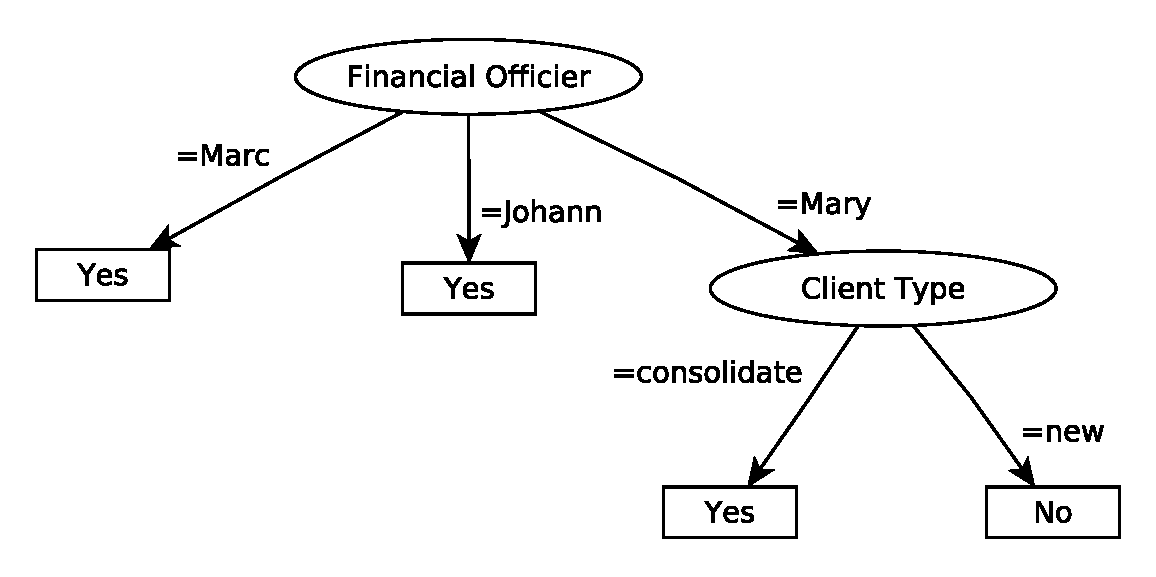
\includegraphics[width=210pt,height=100pt]
{./items/Sales_tree.pdf}
\caption{Decision tree for the conformance analysis.}
\label{salesDecTree}
\end{figure}
The resulting decision tree describes a data pattern in correspondence to which a process instance could present conformance errors: order managed by the sales manager \emph{Mary} and received from consolidate clients of the organization may not respect the standard sales procedure. To get more significant information for our analysis, it is useful to relate what is noticed by the decision tree with the log replay results. Figure \ref{replayResult} presents a Petri net that summarizes the conformance analysis conducted on instances recorded in the event log taken in exam. Arcs are labeled with the number of activations done. Places, whenever they present some remaining or missing tokens, are labeled with the number of these tokens.
\begin{figure}[h]
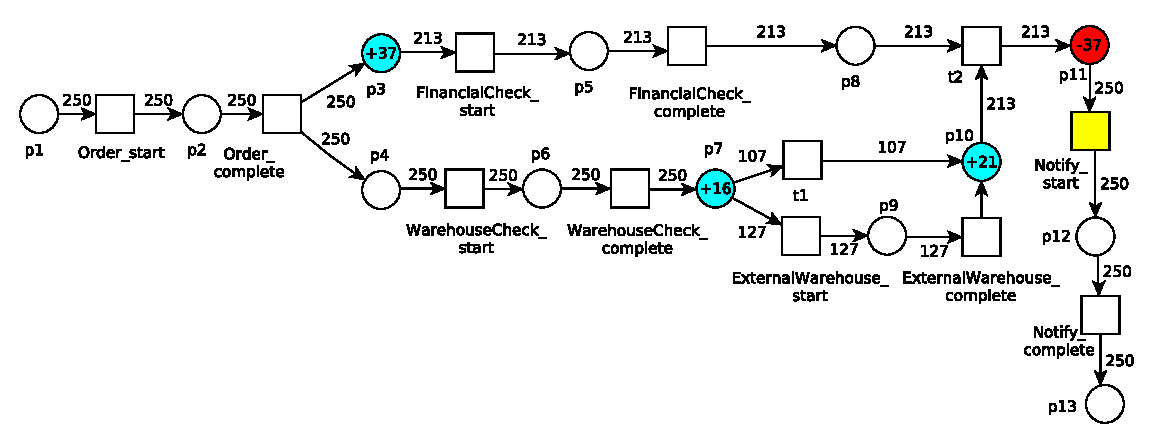
\includegraphics[width=360pt]
{./items/Sales_PN_resultMod.pdf}
\caption{Petri net: conformance results.}
\label{replayResult}
\end{figure}

The Petri net in Figure \ref{replayResult} shows that there are 37 out of 250 process executions with conformance errors. The presence of 37 missing tokens in $p11$ signals a forced execution of  transition \emph{Notify\_start}. In order to provide an interpretation for this results, we have to take into account the non-blocking behavior of the log replay algorithm. In this case, the 37 missing tokens in $p11$ certifies that during the replay the algorithm needs to mimic the event \emph{Notify\_start} but the transition associated to the event is not enabled in the marking reached by the net, so the algorithm creates artificial tokens for completing the trace replay. This situation is possible only if the invisible transition $t2$ is not enabled. Now, if $t2$ is not enabled that means that there are no tokens in the places $p8$ or $p10$. But notice that there are 21 remaining tokens in the place $p10$, so the transition $t2$ is not enabled for those $37$ instances because the place $p8$ does not have any token. Moreover, the Petri net in Figure \ref{replayResult} shows 37 remaining tokens in place $p3$, so we can deduce that in those instances financial activities were not performed. From these facts, we can conclude that the conformance problems presented in  37 instances are due to a missing execution of the financial activity checking. On the other hand, the decision tree reports that the instances with conformance problems are made by consolidate clients.

From the analysis done for the sales process based on both classification and log replay results, a new scenario of the sale procedure has emerged: orders done by the consolidate clients of the organization are not checked from a financial point of view. This fact can be accepted as a possible and reasonable behavior in a sale procedure, consequently an extension of the business process model is needed in order to include the new scenario (\emph{model extension activity}). Alternatively, the new scenario can be considered as an anomaly in the sales procedure. In this case, since the analysis done provides accurate information about the conformance error, corrective measures can be taken in order to avoid errors in the next orders.

The classifier constructed with this approach can be used also in a predictive way. Given a new trace recording a process execution, in order to perform the conformance checking to the process model, the decision tree can be used to predict the conformance result. This bring an advantage in terms of the time required by the analysis since the log replay algorithm takes more time than the one needed by a decision tree to classify a new instance. Moreover, it is worth noting that whenever the set of attributes needed for the classification is known before the completion of a process execution, it can be interesting to predict the conformance result of the execution and avoid the errors that could possibly happen.

\subsection{Extension of the approach for Performance Analysis}\label{ClassPerf}
<<<<<<< HEAD

Performance analysis of a process can be carried exploiting log replay. Since a log contains timestamps, during the replay of a trace it is possible to compute (for each place of the Petri net model) some performance measures such as: \emph{synchronization time} (i.e. time interval between arrival of a token in the place and enabling of a transition in the post-set of the place), \emph{sejour time} (i.e. the time interval between arrival and departure of tokens) and \emph{waiting time} (i.e. the time interval between enabling of a transition in the post-set of the place and token departure).

Performing an analysis based on the measures computed by log replay gives just a \emph{quantitative} information about the process performance. In order to understand the \emph{causes} of performance anomalies that can affect the process behavior, one can explore the process data. Discovering how data attribute can influence process performance provides useful information in analyzing and optimizing the process services. For example, discovering data patterns in correspondence to which some activities need more time for completion than others, helps in making decisions about resources distribution to the process activities or in scheduling activities. In addition to the completion time, one could analyze a process under more complex performance metrics such as the synchronization time. A process with parallel branches and synchronizations can present bottleneck activities that lead to increase the execution time of other activities and consequently the completion time of the entire process. To find out the possible data influences on synchronization time, the approach presented in Section \ref{ClassConformance} for conformance analysis through classification can be easily extended to performance analysis. For example, a classification problem can be formulated for each synchronization point of the process. In this way, the classifier obtained in correspondence to a synchronization point classifies the process instances based on their attribute value and regarding the synchronization time of the point taken into exam. 
=======
Discovering how data attribute can influence process performance provides useful information in analyzing and optimizing the process services. For example, discovering data patterns in correspondence to which some activities need more time for completion than others, helps in making decisions about resources distribution to the process activities or in scheduling activities. In addition to the completion time, one could analyze a process under more complex performance metrics such as the \emph{synchronization time}. A process with parallel branches and synchronizations can present bottleneck activities that lead to increase the execution time of other activities and consequently the completion time of the entire process. To find out the possible data influences on synchronization time, the approach presented in Section \ref{ClassConformance} for conformance analysis through classification can be easily extended to performance analysis. For example, a classification problem can be formulated for each synchronization point of the process. In this way, the model obtained in correspondence to a synchronization point classifies the process instances based on their attribute value and regarding the synchronization time of the point taken into exam. 
>>>>>>> guancio

\begin{comment}
\begin{table}[!h]
\scriptsize
\centering
\begin{tabular}{|p{1cm}|p{1cm}|p{1,5cm}|p{1cm}|p{1,3cm}|p{1,4cm}|p{1,1cm}|p{1,2cm}|p{1,5cm}|}
\hline OrdIde & CltIde & CltType & SalMan & FinOff & WrhsMan & Supplier & OrdResut & Synch\\
\hline
1 & 20 & consolidate & Marco & Alessandro & Alex & Gianni & positive & high\_wareh.\\
\hline
2 & 15 & new & Anna & Mario & Alessio & Mario & positive & normal\\
\hline
3 & 10 &consolidate & Maria & Roberto & Alessio & Mario & negative & normal\\
\hline
2 & 15 & new & Anna & Mario & Roberto & Gianni & positive & high\_wareh.\\
\hline
... & ... & ... & ... & ... & ... & ... & .... & .... \\
\hline
\end{tabular}
\caption{Dataset for the performance analysis.}
\label{tab:SaleDataPerf}
\end{table}
\normalsize

To discover how the process data may influence its performance in term of synchronization time, a classification problem is formulated for each synchronization point of the process. In this way, the model obtained in correspondence to a synchronization point classifies the process instances based on their attribute value and regarding the synchronization time of the point taken into exam. For the sales process presented in Section \ref{example}, a single point of synchronization is identified. In fact, the Petri net in Figure \ref{pnet} has two parallel branches, one for the financial activity and the other for the warehouse activities. We are interested in analyzing the synchronization between these branches. Indeed, the synchronization time of interest is measured in correspondence to the places $p(8)$ and $p(10)$: $tsc(p8)$, $tsc(p10)$ which are computed by the log replay algorithm as explained in Section \ref{Background}.

To formulate the classification problem the dataset is extracted from the event log, whereas the target attribute is one of the log replay performance results. The target must be something that characterizes the performance in term of synchronization. An idea can be to simply consider the difference between synchronization time of $p8$ and $p10$: $tsc(p8) - tsc(p10)$. It should be noted that classification deals with discrete or categorical target attribute. Since the performance metrics, the synchronization time in this case, are expressed as continous values, a discretization phase is required  during the formulation of the classification problem. Let us choose the attribute target as a categorical attribute: given a treshold $S$, if $|tsc(p8)- tsc(p10)|$ exceeds the value $S$, then the target attribute indicates the branch with the high synchronization time, otherwise the target indicates that the instance presents a normal synchronization time. Therefore, the target attribute can assume three possible values: \emph{high\_financial, high\_warehouse} and \emph{normal}. Based on the process data extracted from the event log and target attribute computed by a discretization of the log replay results, the dataset for the classification problem is built and presented in Table \ref{tab:SaleDataPerf}. As done for conformance analysis, the dataset is used as input of the classification algorithm that returns the decision tree presented in Figure \ref{salesPerfDecTree}.

\begin{figure}[h]
\centering
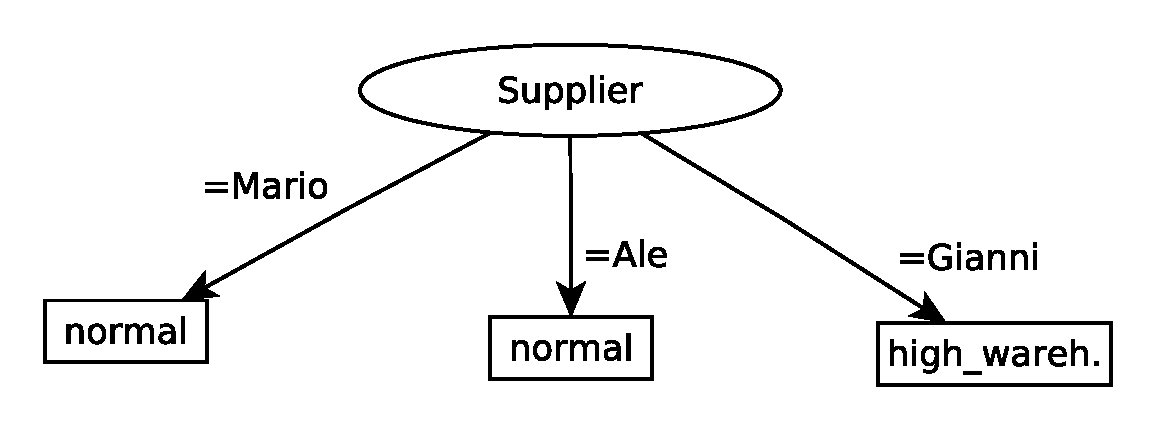
\includegraphics[width=120pt,height=60pt]
{./items/Sales_perf_tree.pdf}
\caption{Decision tree for the performance analysis.}
\label{salesPerfDecTree}
\end{figure}

The decision tree shows that the synchronization time is too high, so not acceptable, for those instances in which the external warehousing is done by the supplier \emph{Gianni}. In other  terms, the rule detected by the decision tree correlates the process performance, measured as the difference of two synchronization times with the external warehousing activities. In this case, the analysis through classification identified such activities as a bottleneck in the \emph{specific case} of the supplier Gianni. This result can be taken as a start point for more investigations that can be done in a \emph{targeted manner} thanks to the pattern identified by the classification analysis. 
\end{comment}

\section{Implementation with ProM}\label{implementation}
In order to experiment with some business process prototypes, the approach presented in this paper has been implemented as a set of plug-ins that integrates \emph{ProM6} \cite{6}, an open-source framework implementing Process Mining tools, and \emph{Weka} \cite{7}, a data mining framework providing machine learning tools.
We can classify the plug-ins developed in three categories. The first one includes plug-ins for building the dataset needed for the classification:
\begin{itemize}
\item \texttt{Generate Instances With Conformance}: this plug-in takes as input an event log and its conformance results computed by log replay. It returns as output a training set as shown in Table \ref{tab:SaleData} in the format needed by Weka classification tool. Note that the plug-in extracts \emph{all} the attributes data recorded in the event log. In case, the dataset resulting can be subject to some \emph{feature selection} techniques before using it as a training set for the classification task.  

\begin{comment}
\item \texttt{Generate Instances With Performance}: the plug-in takes as input an event log, an indication of the synchronization point to examine and the performance result computed by the log replay. The output is a training set as presented in Table \ref{tab:SaleDataPerf}.
\end{comment}

\item \texttt{Generate Instances to Classify}: given an event log, the plug-in generates a dataset of instances that can be classified using a classification model.
\end{itemize}
The second category includes plug-ins for the classifier generation and utilization as a predictive model:
\begin{itemize}
\item \texttt{Generate Classifier}: given a training set, the plug-in generates a decision tree model using $J48$ algorithm, an implementation of the algorithm $C4.5$ developed by Weka.
\item \texttt{Classify Instances}: given a set of non-classified instances and a classifier model, this plug-in simply classify the instances according to the classifier.
\end{itemize}
Finally, the last category includes a set of plug-ins useful for the serialization, deserialization and visualization of the resources used by the previous plug-ins, such as dataset and classifiers. 

\subsection{Methodology}
This last paragraph is dedicated to a description of the methodology to be followed to analyze a business process under the approach presented in this paper.

It should be clear that the analysis presented on the previous Section assumes the presence of a Petri net model of the business process to be analyzed. The model can be expressed in BPMN language as well, but in this case a transformation into a Petri net can be done through the techniques described in \cite{2}. The classification analysis  needs also an event log tracing the process behavior over multiple instances. Given a process model $M$ and an event log $L$, the methodology to be followed for the conformance analysis with the approach presented in Section \ref{ClassConformance} can be summarized by these steps:
\begin{enumerate}

\item \label{step1} \textbf{Log replay analysis}: this phase consists in an execution of the log replay with  the model $M$ and the log $L$ as inputs. The results consists in two structures characterizing both the conformance and the performance of the traces in $L$. Let us call them $ConfResult$, and $PerfResult$.

\item \label{step2} \textbf{Training set construction}: this phase aims to build the training set for the classification technique. This is done through an execution of the plug-in \texttt{Generate Instances With Conformance} with the event log $L$ and the conformance result $ConfResult$ as inputs. Let us call the training set obtaind $TS$.

\item \textbf{Classifier building}: in this step the classification model (decision tree) for the conformance analysis is built using the plug-in \texttt{Generate Classifier} with the training set $TS$ as input. Let us call the decision tree obtained $DT$.

\item \textbf{Using the classifier}: in this step the goal is to exploit $DT$ and the log replay result $ConfResult$ to establish the corrective measures in case of anomalies. Note that both $DT$ and $ConfResult$ can be visualized as in Figures \ref{salesDecTree} and \ref{replayResult} into ProM6 thanks to the plug-ins for resources managing that integrate the framework. $DT$ can also be used in a predictive way to establish the conformance of new process instances without needing a log replay execution. Given an event log containing new process instances, a dataset can be built through the plug-in \texttt{Generate Instances to Classify} and then classified by the plug-in \texttt{Classify Instances} according to the model $DT$.
\end{enumerate}

To perform a performance analysis based on the extension presented in Section \ref{ClassPerf}, the same methodology can be followed modifying the step \ref{step2}. The construction of the training set is done through a plug-in (analogous to \texttt{Generate Instances With Conformance}) that takes as input $PerfResult$ obtained by the step \ref{step1} and an indication about the synchronization point chosen for the analysis.

\addcontentsline{toc}{chapter}{Bibliography} 
\bibliography{biblio}
\bibliographystyle{abbrv} 

\end{document}

